\documentclass{article}

% Language setting
% Replace `english' with e.g. `spanish' to change the document language
\usepackage[english]{babel}

% Set page size and margins
% Replace `letterpaper' with `a4paper' for UK/EU standard size
\usepackage[letterpaper,top=2cm,bottom=2cm,left=3cm,right=3cm,marginparwidth=1.75cm]{geometry}

% Useful packages
\usepackage{amsmath,amsthm,amssymb,amsfonts,graphics}
\usepackage{graphicx}
\usepackage[colorlinks=true, allcolors=blue]{hyperref}
\usepackage{hyperref}
\usepackage{tikz}
\usepackage{circuitikz}
\usepackage{svg}
\usepackage{float}

\title{VLSI Final Project\\
\vspace{10pt}
\large Sine Function Generator\\ \\
\textit{"The sun never sets on the Skywater empire."}}
\author{Ian Eykamp and Joseph Gilbert}

\begin{document}
\maketitle

\section{Overview}
\subsection{Preface}
We had budgeted 30 hours over the last two days of the project preceding the assignment deadline to implement the final stages of the project, including creating the combinational logic by hand once we determined that \emph{qflow} was not worth pursuing any further. One of our computer's kernels completely broke down during this process, which left us with only a single computer to work on. Since we only had one computer between us, we could not work in parallel, and so a project that was expected to take 30 hours took approximately 60 hours over the timespan of 72 hours. We achieved this throughput by parallelizing our respective sleep and work processes and allocating alternating shifts for sleeping and working so that the single computer was running nonstop. 

\subsection{Summary}
The goal of this project is to create a sine wave generator using direct digital synthesis. Our circuit receives as inputs a $100MHz$ clock signal, the power rails, and various ideal current sources for bias references. The major components are the phase counter, combinational logic to approximately compute the sine function, current-steering digital to analog converter (DAC), and output stage which consists of current difference, IV conversion, and filtering using a switched capacitor op amp circuit. For each module, we simulated the circuit in Xschem, laid it out in Magic, and performed layout versus schematic (LVS) verification using Netgen.

\section{Phase Counter}

The phase counter receives a clock signal as input and outputs a 7-bit number representing the phase of the sine wave. A key insight is that when counting up from zero in binary, each bit oscillates between zero and one with half the frequency of the next less significant bit. For example, in the sequence $[000, 001, 010, 011, 100, 101, 110, 111]$, the least signficant bit oscillates every clock cycle, the middle bit oscillates every two clock cycles, and the most significant bit oscillates every four clock cycles. This means we can implement a binary counter simply with a series of cascaded stages that divide the frequency by two.\\

Specifically, for each bit in the counter, we use a flip-flop that toggles state on the rising edge of the clock, and we feed the $\bar{Q}$ output of the $(i-1)^\text{th}$ bit into the clock input of the $i^\text{th}$ register. This divides the clock down by a factor of two for ever flip-flop, since the output will only change state on the rising (or falling) edge of the input. Thus for every down, up cycle of the $(i-1)^\text{th}$ bit, the $i^\text{th}$ bit will go either up or down.
\begin{figure}
    \centering
    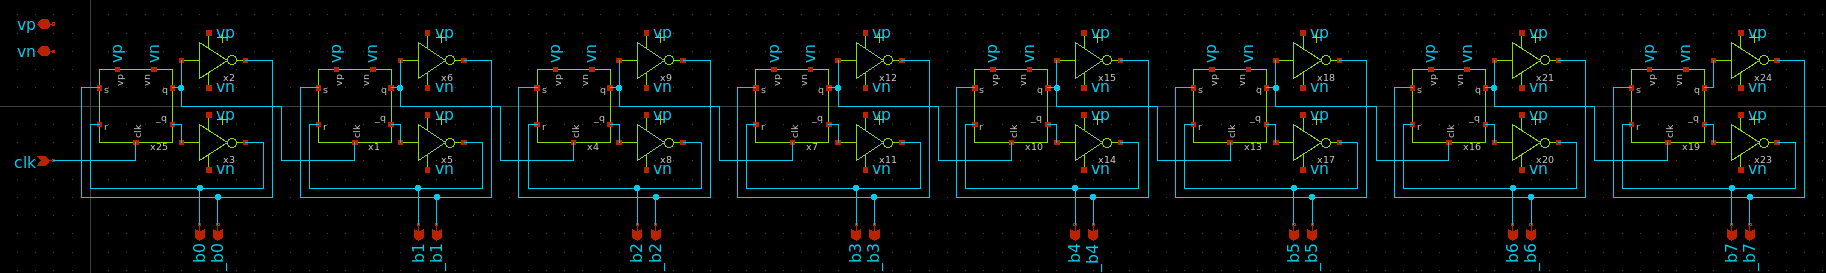
\includegraphics[width=1.0\linewidth]{images/phase_counter_schematic.png}
    \caption{LDS for the phase counter}
    \label{fig:enter-label}
\end{figure}
we originally started with the csrl flip flop but it ended up being to sensitive to implement reliably with our high frequencies. so we ended up opting for a more standard sr-latch based flip flop with the downside of less accurate timings.
\begin{figure}
    \centering
    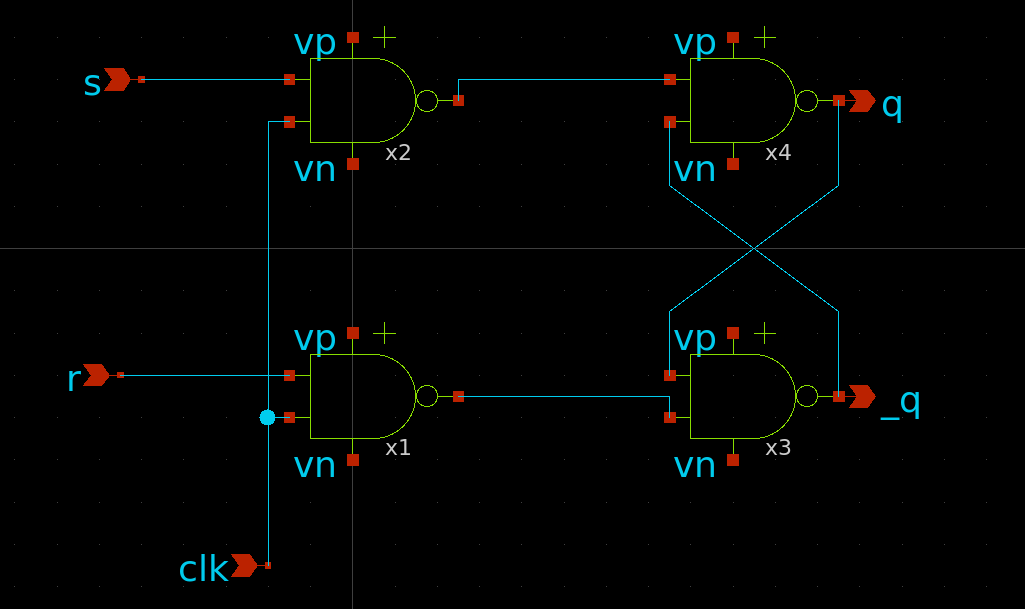
\includegraphics[width=0.5\linewidth]{images/sr_latch.png}
    \caption{SR latch design using nand gates}
    \label{fig:enter-label}
\end{figure}
\begin{figure}
    \centering
    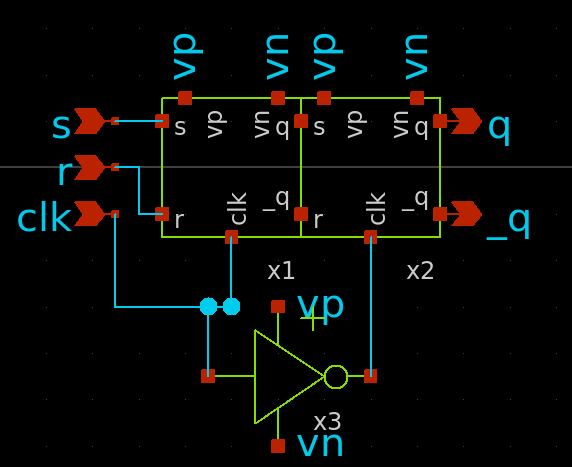
\includegraphics[width=0.5\linewidth]{images/edge_triggered_flip_flop.png}
    \caption{SR latch based flip flop design}
    \label{fig:enter-label}
\end{figure}

\section{Combinational Logic}
A direct digital synthesis method for producing an irrational function such as sine necessarily involves some kind of non-elegant combinational logic, such as a lookup table or some arbitrary mathematical function that approximate the values in the lookup table. We chose the former method.\\

We used a python script to generate the values for when each of the bits should be on or not and then used sympy to calculate the boolean algebra. this gave us the equations \begin{equation} \label{eq1}
\begin{split}d_0 = \neg b_{0},\end{split}
\end{equation}

\begin{equation} \label{eq2}
\begin{split}d_1 = b_{0} \veebar \left(\left(b_{1} \wedge \neg b_{2}\right) \vee \left(b_{2} \wedge \neg b_{1}\right) \vee \left(b_{2} \wedge \neg b_{3} \wedge \neg b_{4}\right) \vee \left(b_{3} \wedge b_{4} \wedge \neg b_{1}\right) \allowbreak \vee \left(b_{3} \wedge b_{5} \wedge b_{6} \wedge \neg b_{1}\right)\right),\end{split}
\end{equation}

\begin{equation} \label{eq3}
\begin{split}
d_2 = b_{0} \veebar & \left(\left(b_{1} \wedge b_{4} \wedge \neg b_{3}\right) \vee \left(b_{1} \wedge \neg b_{2} \wedge \neg b_{4}\right) \allowbreak \vee \left(b_{2} \wedge b_{4} \wedge \neg b_{1}\right) \vee \left(b_{2} \wedge b_{5} \wedge \neg b_{1}\right) \allowbreak\\* & \vee \left(b_{3} \wedge \neg b_{4} \wedge \neg b_{5}\right) \allowbreak \vee \left(b_{3} \wedge \neg b_{4} \wedge \neg b_{6}\right) \allowbreak \vee \left(b_{4} \wedge b_{5} \wedge \neg b_{3}\right)\right),\end{split}
\end{equation}

\begin{equation} \label{eq4}
\begin{split}d_3 = b_{0} & \veebar \left(\left(b_{2} \wedge b_{3} \wedge \neg b_{1}\right) \allowbreak \vee \left(b_{1} \wedge b_{2} \wedge b_{4} \wedge \neg b_{3}\right) \allowbreak \vee \left(b_{1} \wedge b_{3} \wedge b_{4} \wedge \neg b_{2}\right) \allowbreak \vee \left(b_{1} \wedge b_{4} \wedge \neg b_{5} \wedge \neg b_{6}\right) \allowbreak\\* & \vee \left(b_{1} \wedge \neg b_{2} \wedge \neg b_{3} \wedge \neg b_{4}\right) \allowbreak \vee \left(b_{1} \wedge \neg b_{2} \wedge \neg b_{3} \wedge \neg b_{6}\right) \allowbreak \vee \left(b_{1} \wedge \neg b_{3} \wedge \neg b_{5} \wedge \neg b_{6}\right) \allowbreak \\* & \vee \left(b_{2} \wedge \neg b_{1} \wedge \neg b_{4} \wedge \neg b_{5}\right) \allowbreak  \vee \left(b_{3} \wedge \neg b_{1} \wedge \neg b_{4} \wedge \neg b_{5}\right) \vee \left(b_{3} \wedge \neg b_{1} \wedge \neg b_{4} \wedge \neg b_{6}\right) \\* &\vee \left(b_{4} \wedge \neg b_{2} \wedge \neg b_{3} \wedge \neg b_{5}\right) \vee \left(b_{2} \wedge b_{3} \wedge b_{5} \wedge b_{6} \wedge \neg b_{4}\right) \vee \left(b_{2} \wedge b_{4} \wedge b_{5} \wedge b_{6} \wedge \neg b_{3}\right) \\* & \vee \left(b_{3} \wedge b_{4} \wedge b_{5} \wedge b_{6} \wedge \neg b_{2}\right) \vee \left(b_{5} \wedge b_{6} \wedge \neg b_{2} \wedge \neg b_{3} \wedge \neg b_{4}\right)\right)\end{split}
\end{equation}

We can however exploit one of the two axes of symmetry in the sine function, based on the fact that the sine of any number can be calculated using only the first $180\deg$. Based on the symmetry of the unit circle, we have $sin(\pi + \theta) = -sin(\theta)$.  Thus, we only need to create combinational logic for the first one hundred eighty degrees of the function, which is all but the most significant bit $\Phi_{n-1}$.\\

Thus, for a 7-bit phase input $\Phi$, our combinational logic needs to calculate the result for bits $\Phi_0$ through $\Phi_4$.\\

\begin{figure}
    \centering
    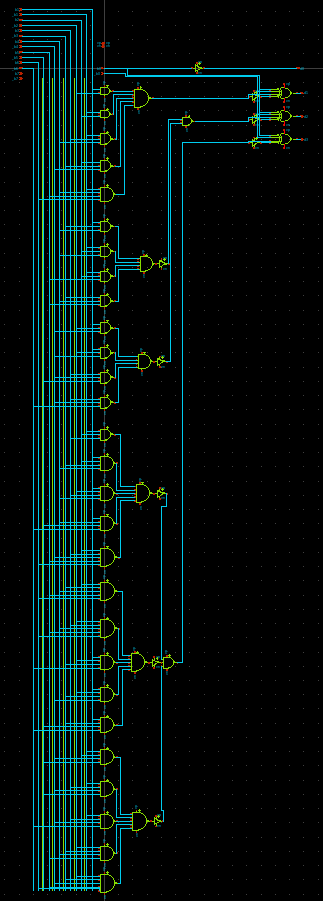
\includegraphics[width=0.5\linewidth]{images/sin_generator_combinational_logic.png}
    \caption{lds for the sin generator}
    \label{fig:lds_sin}
\end{figure}

This combined with the phase counter generated a sin wave albeit with some amount of noise 
\begin{figure}
    \centering
    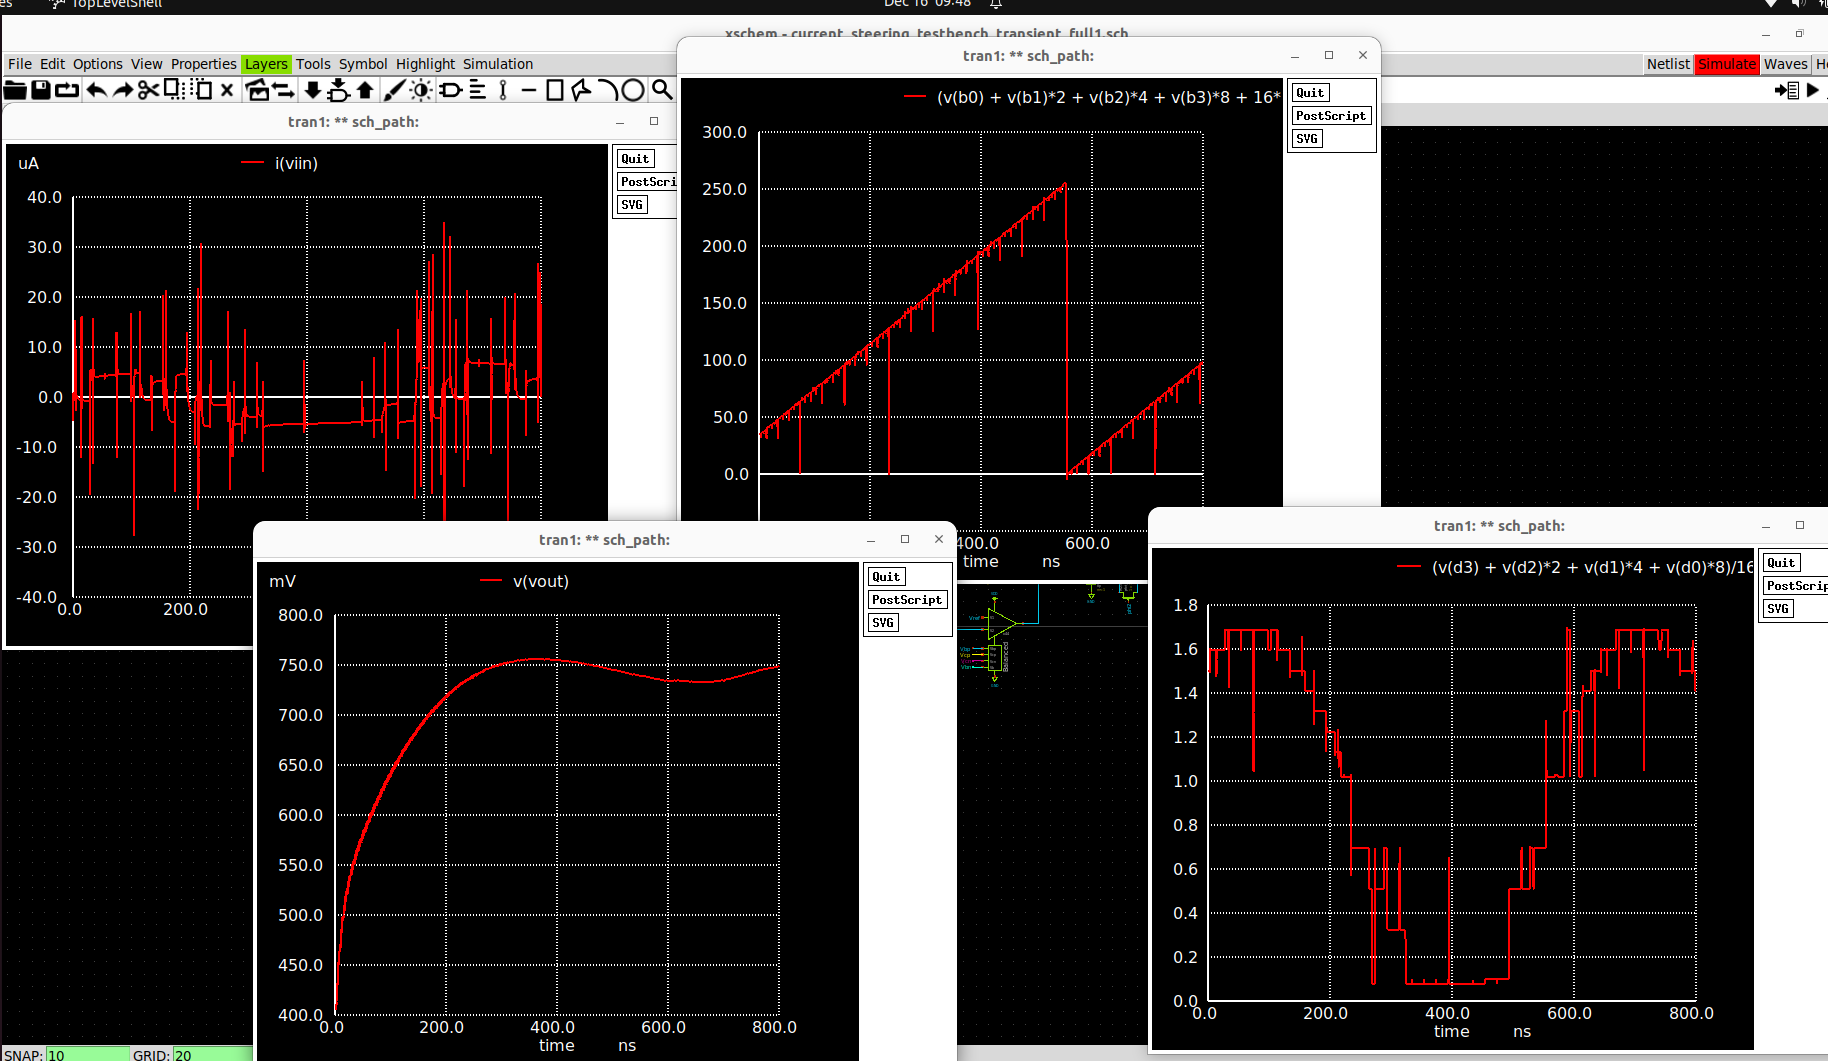
\includegraphics[width=0.8\linewidth]{images/preliminary_combinational_logic_results.png}
    \caption{top left: the current output from the DAC. top middle: counter output. bottom left voltage output of signal (it started with the output cap fully discharged). bottom right: binary DAC input.}
    \label{fig:lds_sin}
\end{figure}

\begin{figure}
    \centering
    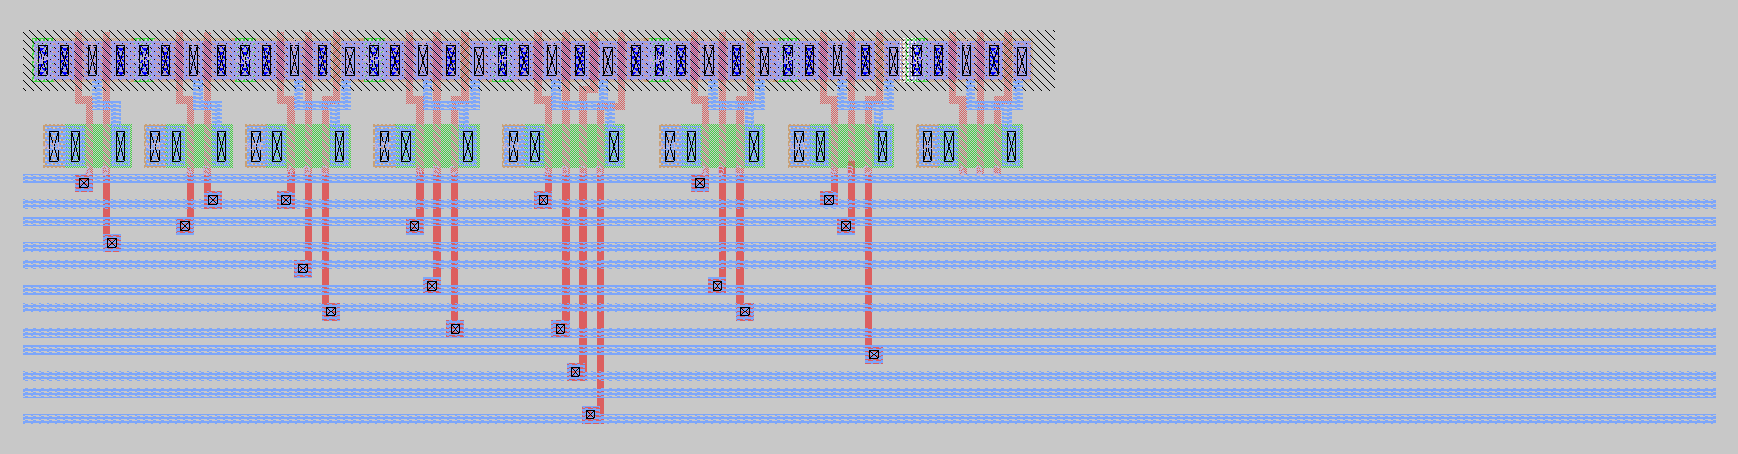
\includegraphics[width=0.8\linewidth]{images/not used yet/nand_tree_cl.png}
    \caption{unfinished layout of the full combinational logic}
    \label{fig:lds_sin}
\end{figure}

our xschem was working but we didnt end up being able to route anything more than a couple of and gates due to magic crashing when we opened the file it was in.




\section{Current-Steering DAC}
\subsection{Digital select signals}
A current steering DAC contains a large number of unit cells which, depending on the code word, pull current from one source or another. The differential current is then proportional to the number of unit cells that were turned on; that is, proportional to the code word. In the most straightforward implementation, each cell has its own control signal; however, we created a grid layout such that each cell can be addressed by its row and column. Each cell has three inputs: row $y$, column $x$, and column $x+1$. The cell is on if either its row and column are on, or if the next column over is on, as expressed in Equation \ref{eq:unit_cell_decoder_boolean_logic}.

\begin{equation}
    \label{eq:unit_cell_decoder_boolean_logic}
    \text{State} = (\text{Row}_y \cap \text{Column}_x) \cup \text{Column}_{x+1}
\end{equation}

For each code word, the row and column truth table is given in Table \ref{tab:4_bit_decoder_truth_table}. For the 4-bit case, it is trivial to construct the row and column signals from the binary input using Equations \ref{eq:4_bit_decoder_logic}, where $b_n$ is the $n^{\text{th}}$ bit of the binary representation of the code word.

\begin{equation}    
    \label{eq:4_bit_decoder_logic}
    \begin{split}
        &\text{Row}_0 = \text{HIGH}\\
        &\text{Row}_1 = b_0 \cup b_1\\
        &\text{Row}_2 = b_1\\
        &\text{Row}_3 = b_0 \cap b_1\\
        &\\
        &\text{Column}_0 = \text{HIGH}\\
        &\text{Column}_1 = b_2 \cup b_3\\
        &\text{Column}_2 = b_3\\
        &\text{Column}_3 = b_2 \cap b_3
    \end{split}
\end{equation}

\begin{center}
\begin{tabular}{ c|c|c|c|c|c|c|c|c|c }
\label{tab:4_bit_decoder_truth_table}
 Input & Code Word & Row 0 & Row 1 & Row 2 & Row 3 & Col 0 & Col 1 & Col 2 & Col 3\\ 
 \hline
 1 &  0000 & 1 & 0 & 0 & 0 & 1 & 0 & 0 & 0 \\
 2 &  0001 & 1 & 1 & 0 & 0 & 1 & 0 & 0 & 0 \\
 3 &  0010 & 1 & 1 & 1 & 0 & 1 & 0 & 0 & 0 \\
 4 &  0011 & 1 & 1 & 1 & 1 & 1 & 0 & 0 & 0 \\
 5 &  0100 & 1 & 0 & 0 & 0 & 1 & 1 & 0 & 0 \\
 6 &  0101 & 1 & 1 & 0 & 0 & 1 & 1 & 0 & 0 \\
 7 &  0110 & 1 & 1 & 1 & 0 & 1 & 1 & 0 & 0 \\
 8 &  0111 & 1 & 1 & 1 & 1 & 1 & 1 & 0 & 0 \\
 9 &  1000 & 1 & 0 & 0 & 0 & 1 & 1 & 1 & 0 \\
 10 &  1001 & 1 & 1 & 0 & 0 & 1 & 1 & 1 & 0 \\
 11 & 1010 & 1 & 1 & 1 & 0 & 1 & 1 & 1 & 0 \\
 12 & 1011 & 1 & 1 & 1 & 1 & 1 & 1 & 1 & 0 \\
 13 & 1100 & 1 & 0 & 0 & 0 & 1 & 1 & 1 & 1 \\
 14 & 1101 & 1 & 1 & 0 & 0 & 1 & 1 & 1 & 1 \\
 15 & 1110 & 1 & 1 & 1 & 0 & 1 & 1 & 1 & 1 \\
 16 & 1111 & 1 & 1 & 1 & 1 & 1 & 1 & 1 & 1 \\
 \hline
\end{tabular}
\end{center}

The unit cell and unit decoder implementing Equation \ref{eq:unit_cell_decoder_boolean_logic} are shown in Figure \ref{}. The binary decoder implementing Equations \ref{eq:4_bit_decoder_logic} is shown in Figure \ref{}. The digital logic is laid out using minimum-width transistors. The transistors for steering the current are large, because they must draw a precise amount of current for the DAC to have a linear response. The cascoded bias transistor is biased using the cascode voltage generator from MP3 and a $0.5\mu A$ external current source.

\begin{figure}[H]
    \centering{}
    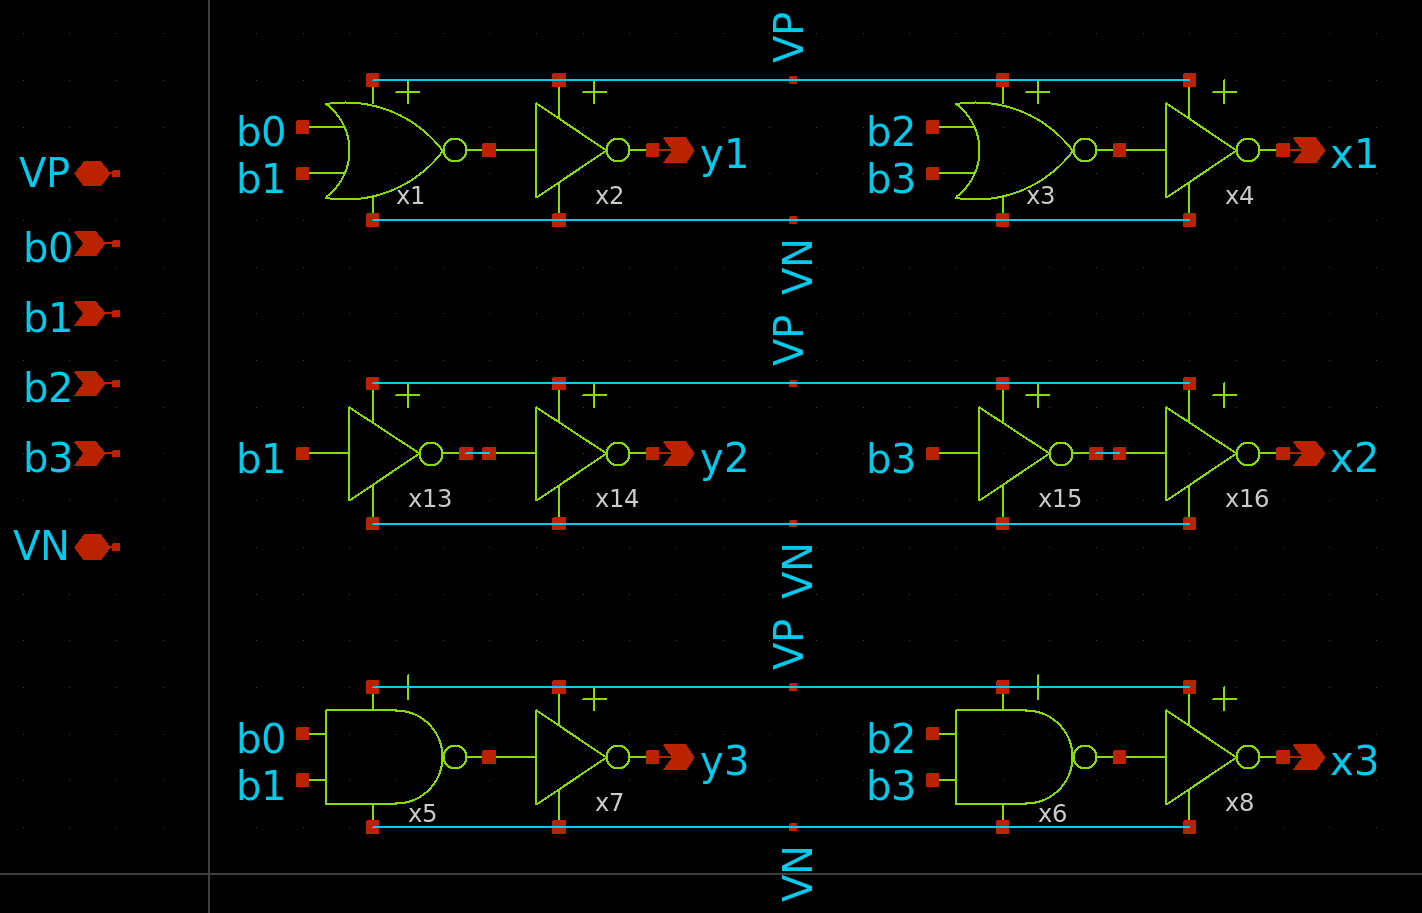
\includegraphics[width=0.7\columnwidth]{images/binary_decoder_block_diagram.png}
    \caption{Schematic representation of binary decoder logic using and gates, or gates, and buffers.}
    \label{fig:binary_decoder_block_diagram}
\end{figure}

\begin{figure}[H]
    \centering{}
    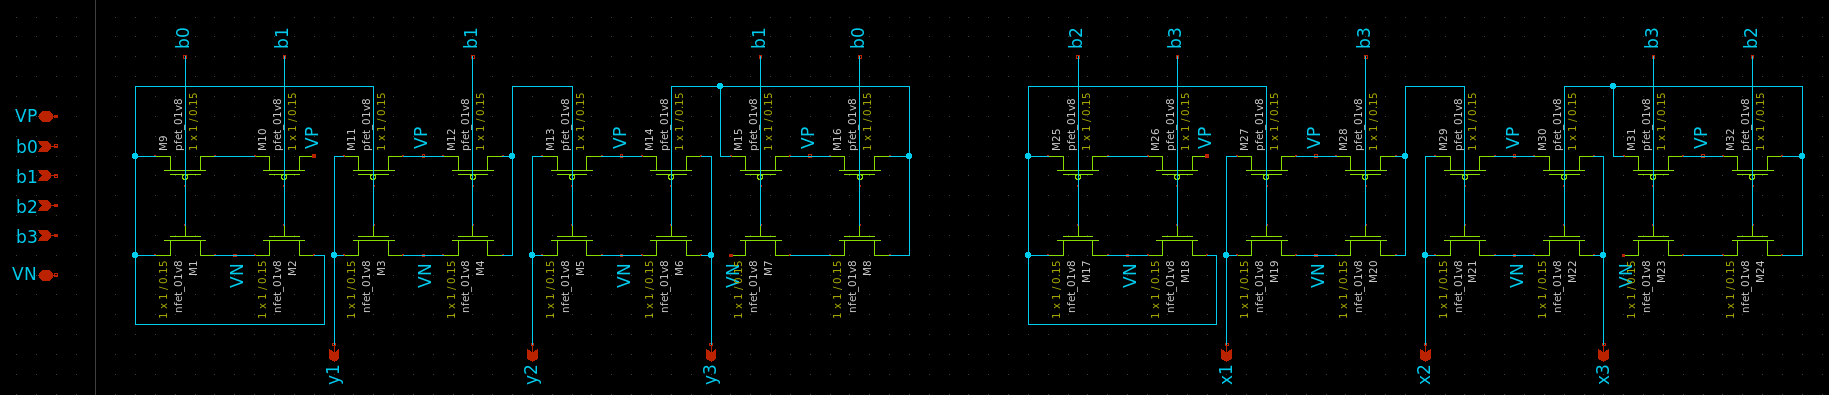
\includegraphics[width=0.7\columnwidth]{images/binary_decoder_schematic.png}
    \caption{Layout driven schematic for binary decoder to generate row and column signals from a 4-bit binary input.}
    \label{fig:binary_decoder_schematic}
\end{figure}

\begin{figure}[H]
    \centering{}
    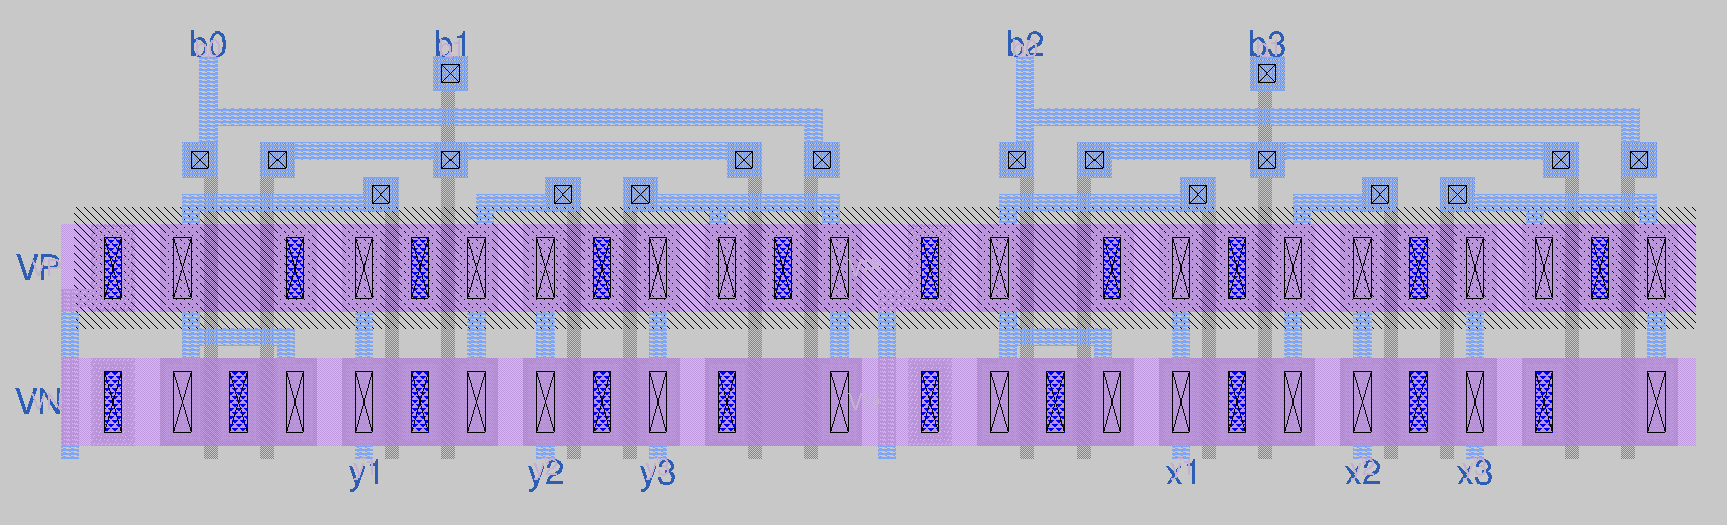
\includegraphics[width=0.7\columnwidth]{images/4_bit_decoder_layout.png}
    \caption{Layout for 4-bit binary decoder.}
    \label{fig:4_bit_decoder_layout}
\end{figure}

\subsection{Layout considerations}
The layout for an individual current steering cell is shown in Figure \ref{fig:unit_cell_schematic}. The layout for the entire DAC, including dummy devices and common centroid mirroring, is shown in Figure \ref{fig:unit_cell_layout}.\\

For the current steering DAC to have a linear response, there must not be much variation in the current drawn by each cell. For a large DAC, this is not guaranteed, since fabrication introduces significant spatial variation in the device. If the variations can be approximated as linear over the length of the device, then we can eliminate these effects if all of our transistors share a common centroid. We accomplish this by duplicating cells of the DAC with a 180 degree rotation and joining cells that are diagonally opposite each other and thus have their centroid where the diagonals meet.\\

Another consideration is that cells near the border of a layout tend to behave differently from those in the middle. We addressed this by including a ring of dummy cells around the entire perimeter. Our final layout consists of a 6x10 grid containing 32 pairwise common-centroided cells and 28 dummy devices. Our design can easily be scaled up to larger grids in which the ratio of usable cells to dummy cells becomes more desirable.\\

\begin{figure}[H]
    \centering{}
    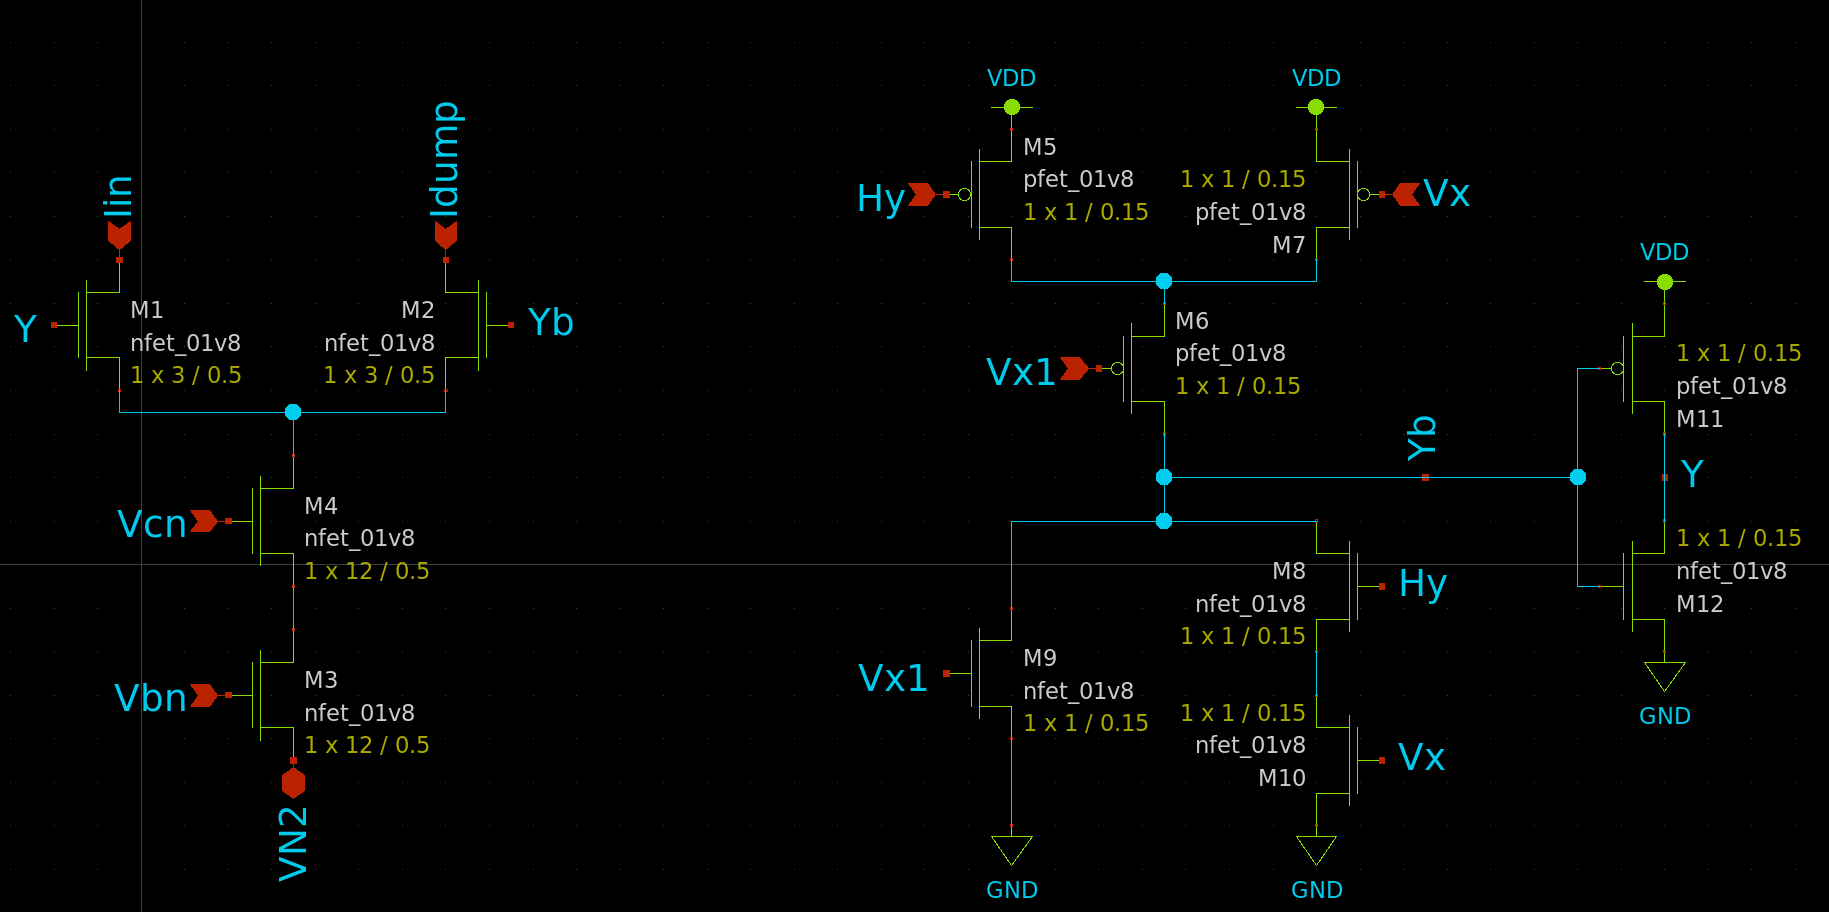
\includegraphics[width=0.7\columnwidth]{images/unit_cell_schematic.png}
    \caption{Unit current steering cell schematic, including current steering and decoding components.}
    \label{fig:unit_cell_schematic}
\end{figure}

\begin{figure}[H]
    \centering{}
    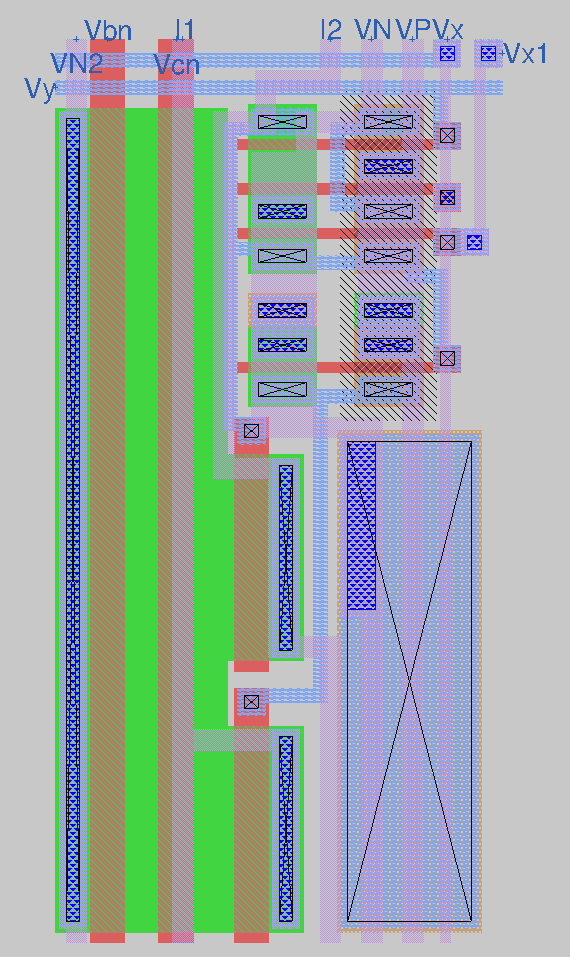
\includegraphics[width=0.7\columnwidth]{images/current_steering_unit_cell_layout.png}
    \caption{Unit current steering cell consisting of analog current steering (large nMOS transistors on the left) and digital decoder logic (minimum width pMOS and nMOS transistors). All signals needed by a cell, including power rails, select signals, current carrying wires, and bias voltages, are propagated through the cell on layers metal 1 and below such that cells near the center of the DAC can access these signals from the peripheries.}
    \label{fig:unit_cell_layout}
\end{figure}

The unit cell layout is designed to propagate all select signals and power busses through the grid without additional routing between cells. Each cell handles no fewer than ten inputs and outputs, and it manages to do so entirely in sub–metal 1 layers.

\begin{figure}[H]
    \centering{}
    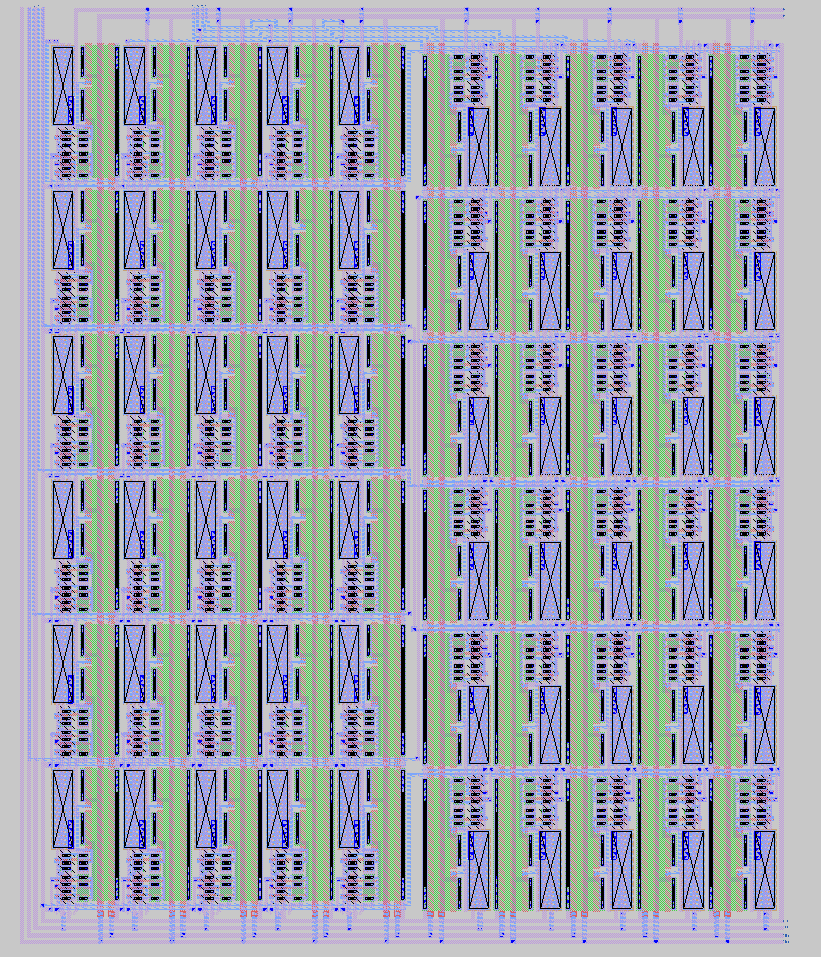
\includegraphics[width=1.0\columnwidth]{images/current_steering_dac_layout.png}
    \caption{Current steering DAC consisting of a grid of sixty unit cells. The inner 4x8 grid is the actual 16-cell DAC, which is mirrored and common centroided across the center line. The outer ring contains dummy cells. The entire DAC is routed in metal 1 and below, which allows for a ground plane in metal 2. Row and column select lines are at the top left of the DAC.}
    \label{fig:dac_layout}
\end{figure}

\section{Output Stage}
The current steering DAC draws a differential current which is proportional to the code word. The output stage turns the differential current into a single-ended output voltage. Our design contains a current difference circuit and a combined IV converter–low pass filter using an op amp switched capacitor circuit.

For the IV converter and low-pass filter, we use the op amp configuration shown in Figure \ref{}. The switched capacitor behaves like a resistor with resistance $R_s = \frac{1}{C_s f_s}$ where $C_s$ is the capacitance of the switched capacitor and $f_s$ is the switching frequency. The impedance of the parallel resistor and capacitor is given in Equation \ref{eq:equivalent_impedance}, where $f$ is the frequency of the signal.

\begin{equation}
    \label{eq:equivalent_impedance}
    Z = \frac{1}{\frac{1}{R_s} + 2 \pi j f C} = \frac{1}{C_s f_s + 2 \pi j f C}
\end{equation}

The cutoff frequency is 

\begin{equation}
    f_0 = \frac{1}{2 \pi j R_s C} = \frac{C_s f_s}{2 \pi j C} = \frac{C_s}{C} \frac{f_s}{2 \pi j}
\end{equation}

The combinational logic produces a sine wave with a period of 128 clock cycles, such that the sine wave frequency is $\frac{f_s}{128}$. We want to target the cutoff frequency of the filter to be roughly the frequency of the sine wave, so that we eliminate the higher frequency error from the stair stepping behavior. Thus, we chose

\begin{equation}
\begin{split}
    \label{eq:capacitor_speccing}
    & f_0 = \frac{C_s}{C} \frac{f_s}{2 \pi j} = \frac{f_s}{128} \\
    & |\frac{C_s}{C}| =\frac{2 \pi}{128} \approx 0.05
\end{split} 
\end{equation}

By Ohm's law, the current to voltage conversion is given by $V = IZ$. For a $\pm 10\mu A$ current, we want a roughly

\subsection{IV converter and low pass filter}
We used a simple op amp circuit using our diff amp from MP3 as a combined current-to-voltage converter and low pass filter. 


\begin{figure}[H]
    \centering{}
    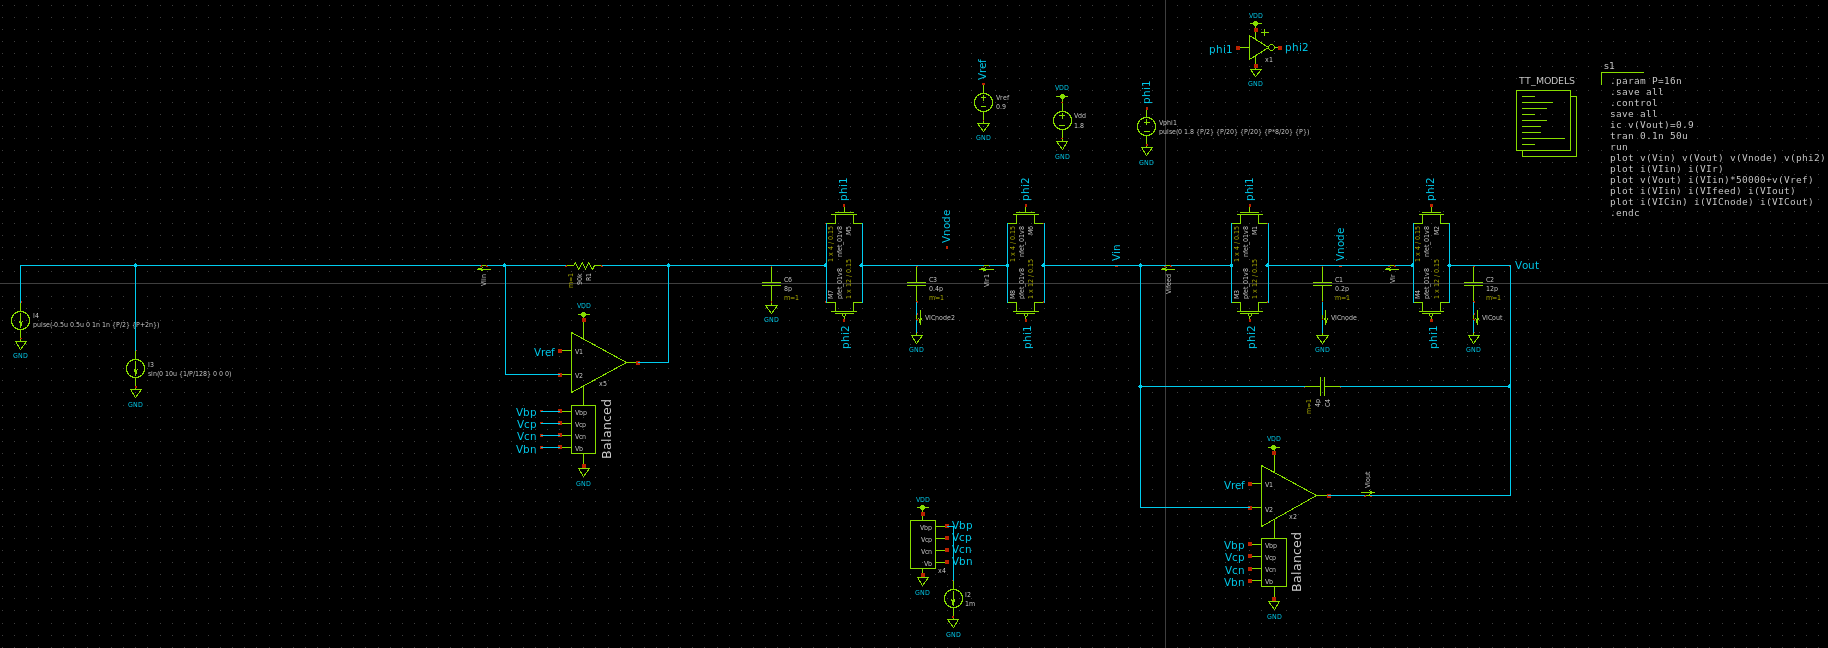
\includegraphics[width=1.0\columnwidth]{images/switched_capacitor_circuit_3.png}
    \caption{Simulation circuit for output stage. The first op amp and resistor act as a current to voltage (IV) converter. The next stage uses two switched capacitor RC circuits to create a second order low pass filter with a corner frequency at the desired sinusoidal output frequency.}
    \label{fig:switched_capacitor_circuit}
\end{figure}

\begin{figure}[H]
    \centering{}
    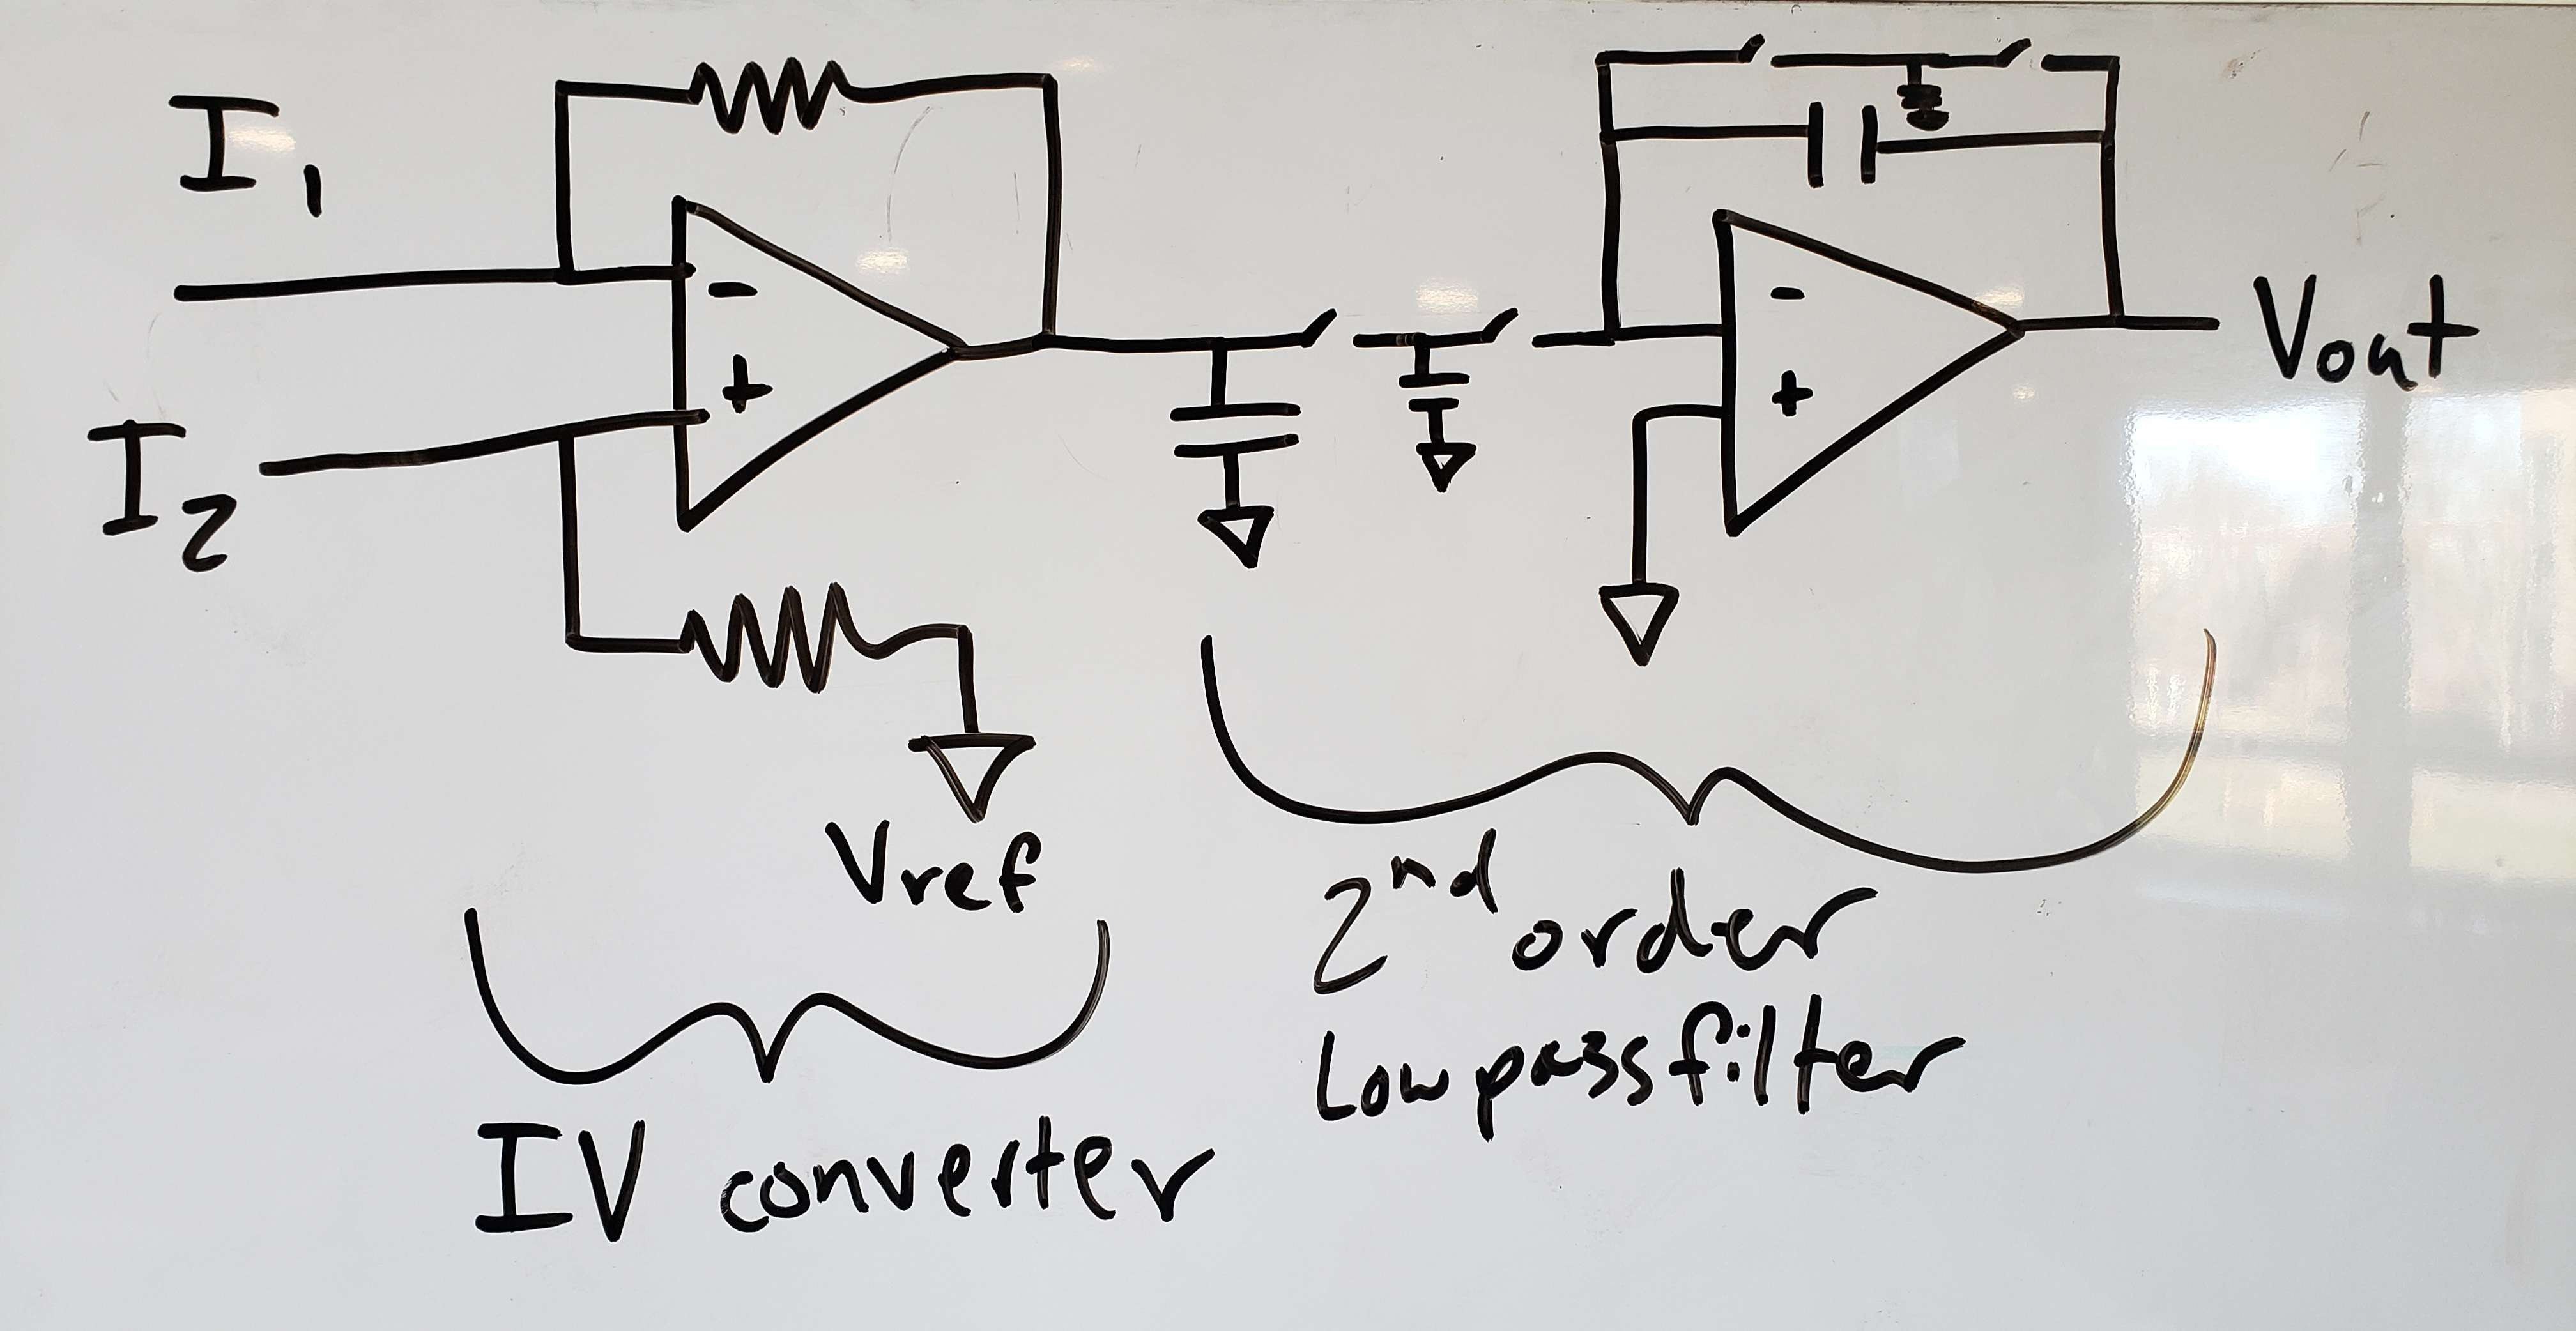
\includegraphics[width=1.0\columnwidth]{images/whiteboard_diagram.jpg}
    \caption{diagram of the differential output stage}
    \label{fig:switched_capacitor_circuit}
\end{figure}


\section{GitHub Files}

All of my files for the final project are in my \href{https://github.com/ianeyk/magic-dds}{GitHub repository} (currently under the branch \emph{main}).

all of the file made with xschem are in the \verb$/xschem/$ folder all of the magic files are in \verb$/magic/$, all of the comp.out files are in \verb$/magic/comp_out/$, and the \verb$/simulations/$ folder contians the python scripts and notebooks that were used to calculate values and layouts.

\section{Additional Figures}

\begin{figure}[H]
    \centering{}
    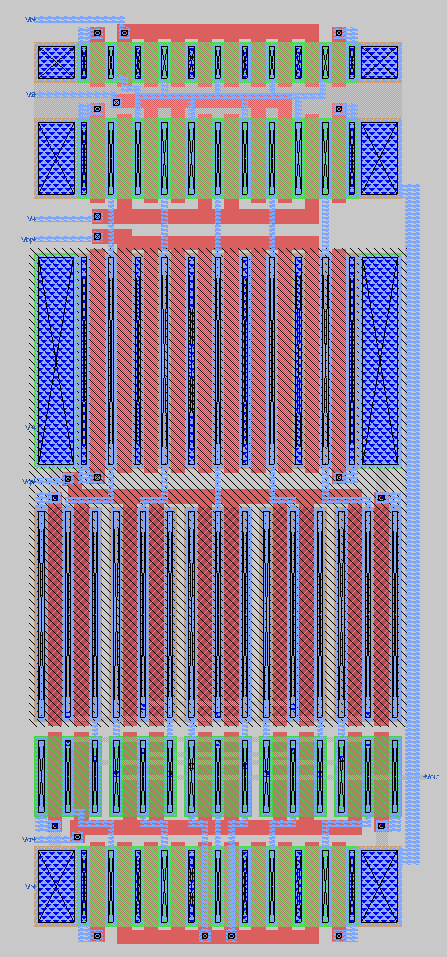
\includegraphics[width=0.5\columnwidth]{images/balanced_op_amp_layout.png}
    \caption{Op amp layout. Slightly modified from Mini-Project 3 to make the pMOS diffusion regions wider. The strength of the pMOS transistors roughly matches the strength of the nMOS transistors.}
    \label{fig:opamp_layout}
\end{figure}

\begin{figure}[H]
    \centering{}
    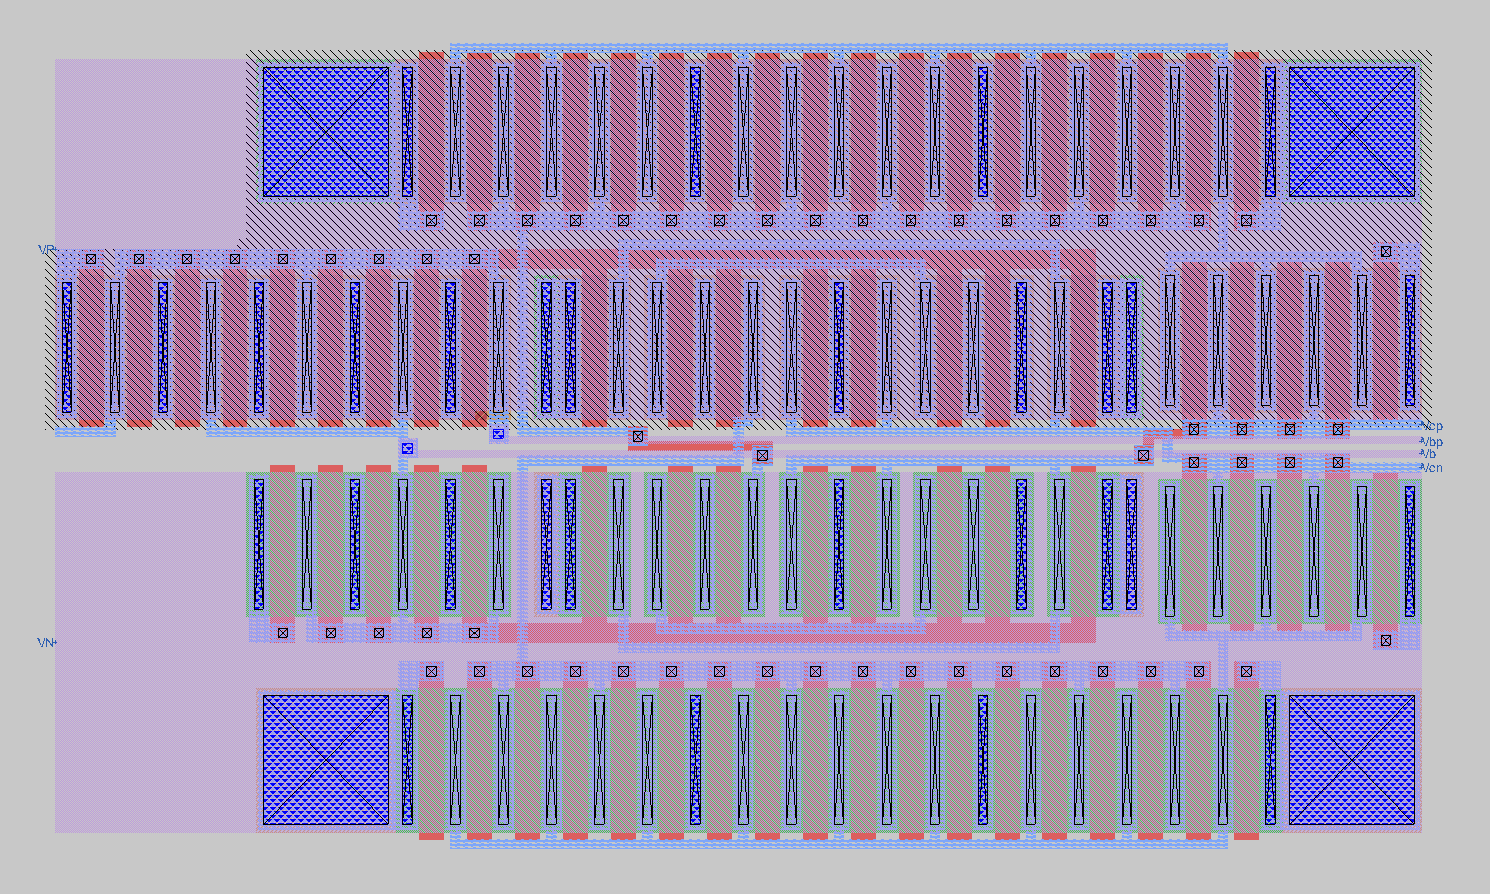
\includegraphics[width=0.7\columnwidth]{images/bias_layout_mp3.png}
    \caption{Cascode bias voltage layout from Mini-Project 3.}
    \label{fig:bias_layout}
\end{figure}

\begin{figure}[H]
    \centering{}
    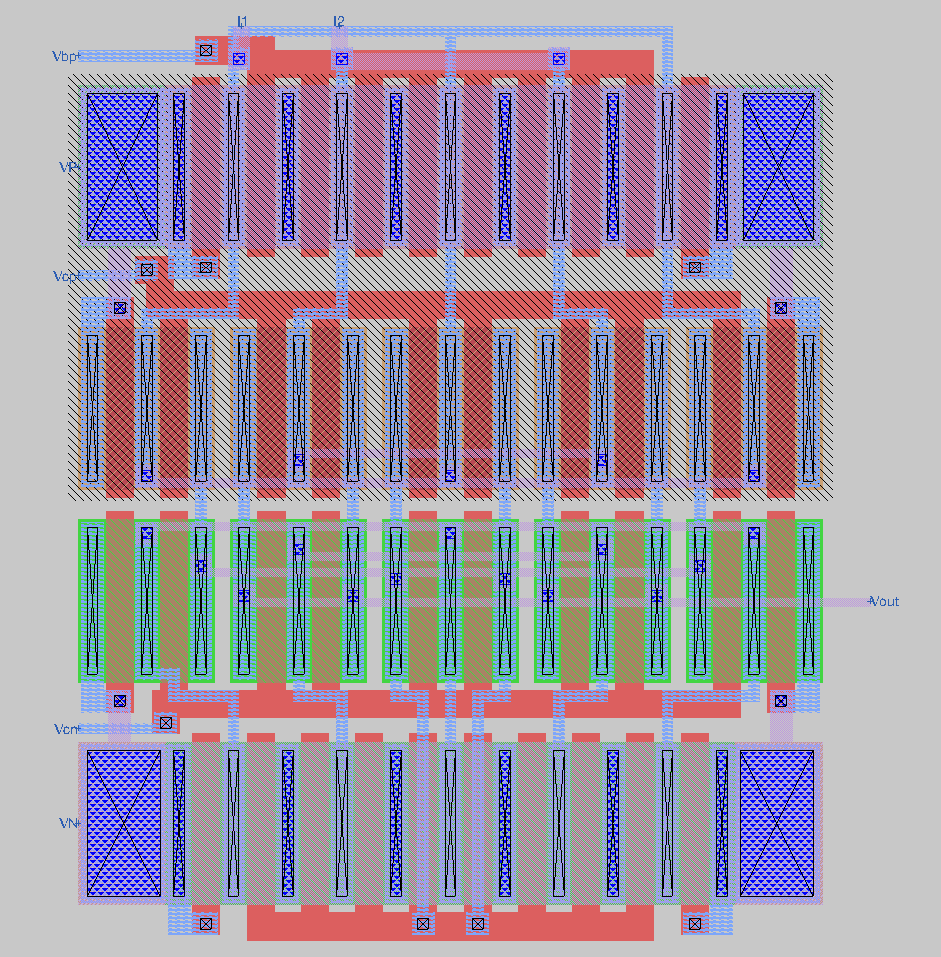
\includegraphics[width=0.7\columnwidth]{images/current_difference_layout.png}
    \caption{Current difference circuit layout. This is a modified version of the op amp from Mini-Project 3 without the differential pair.}
    \label{fig:current_difference_layout}
\end{figure}

\begin{figure}[H]
    \centering{}
    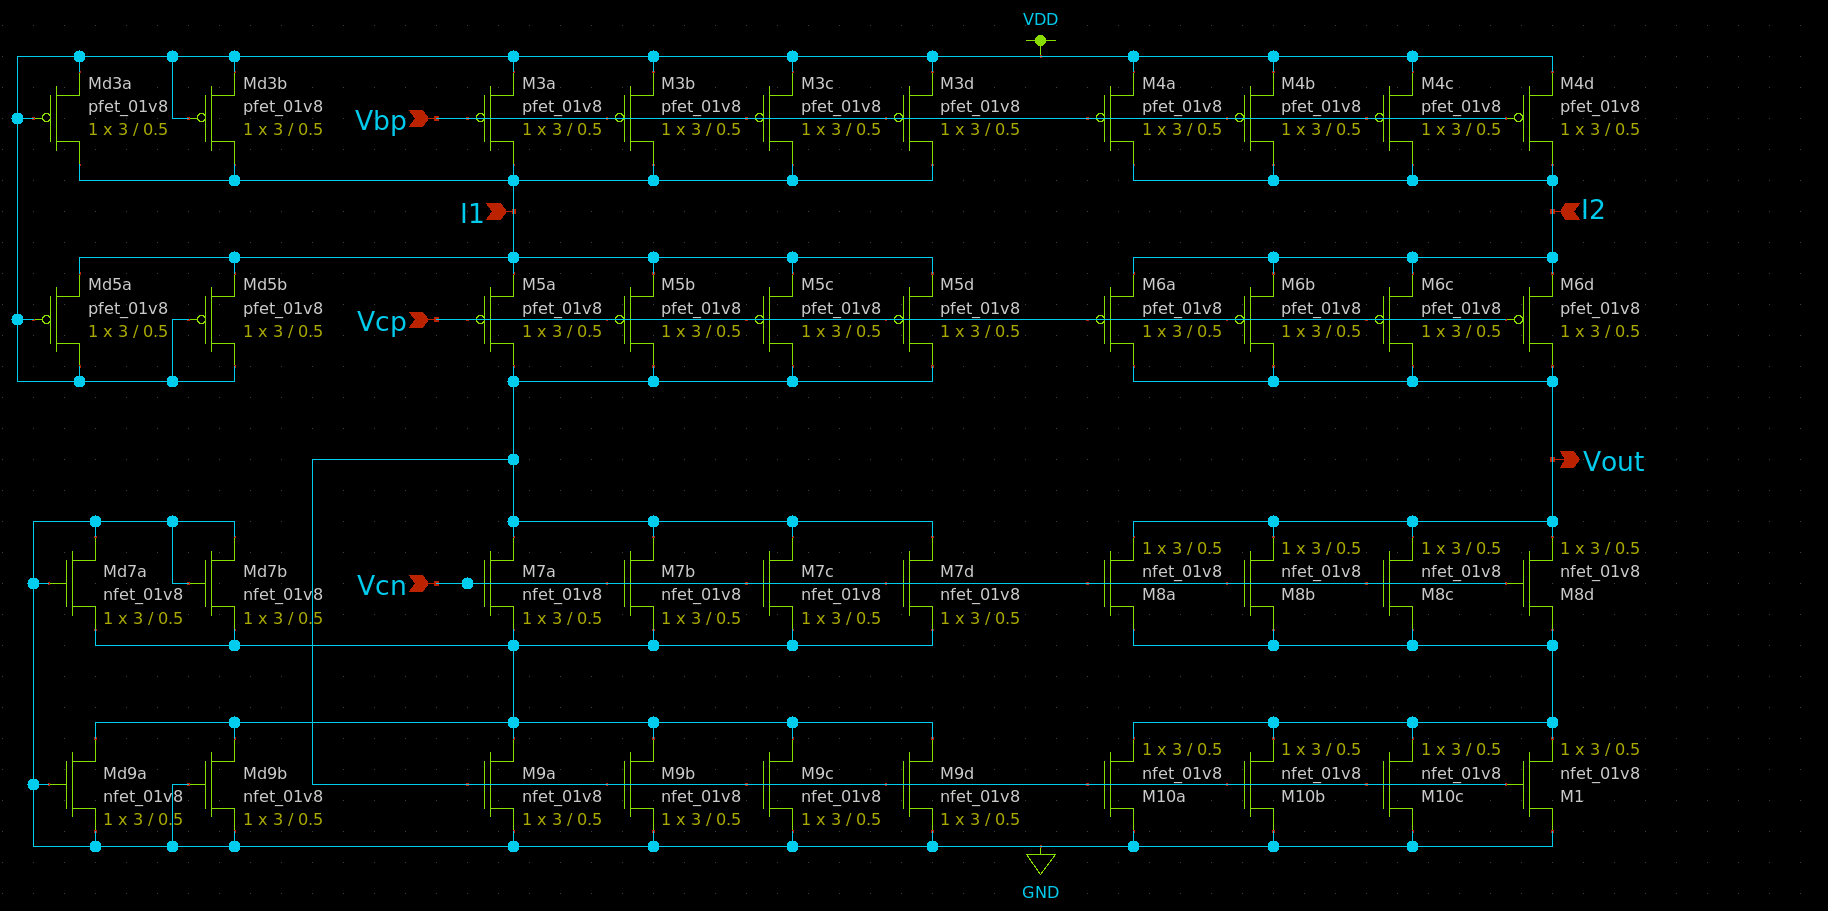
\includegraphics[width=0.7\columnwidth]{images/current_difference_lvs_schematic.png}
    \caption{Current difference layout-driven schematic. This is a modified version of the op amp from Mini-Project 3 without the differential pair.}
    \label{fig:current_difference_schematic}
\end{figure}

\begin{figure}[H]
    \centering{}
    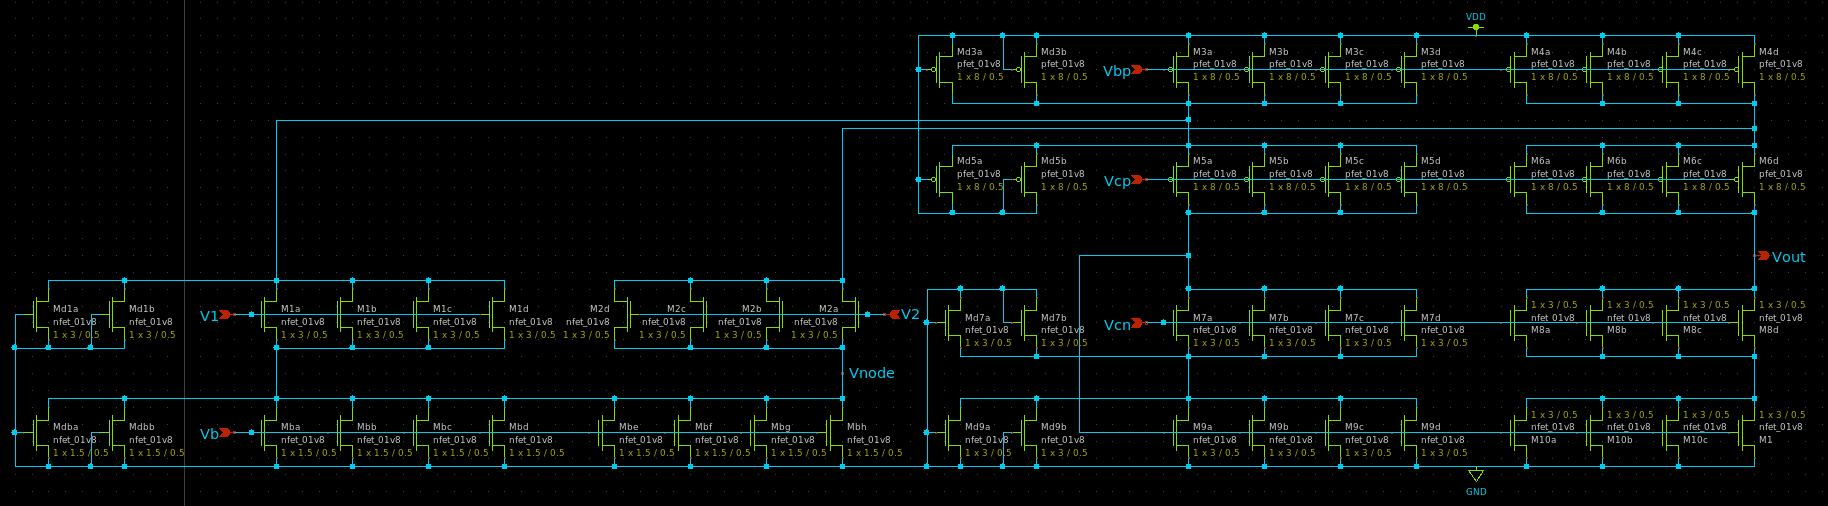
\includegraphics[width=0.7\columnwidth]{images/opamp_lvs_schematic.png}
    \caption{Op amp layout. Slightly modified from Mini-Project 3 to make the pMOS diffusion regions wider. The strength of the pMOS transistors roughly matches the strength of the nMOS transistors.}
    \label{fig:opamp_schematic}
\end{figure}

\begin{figure}[H]
    \centering{}
    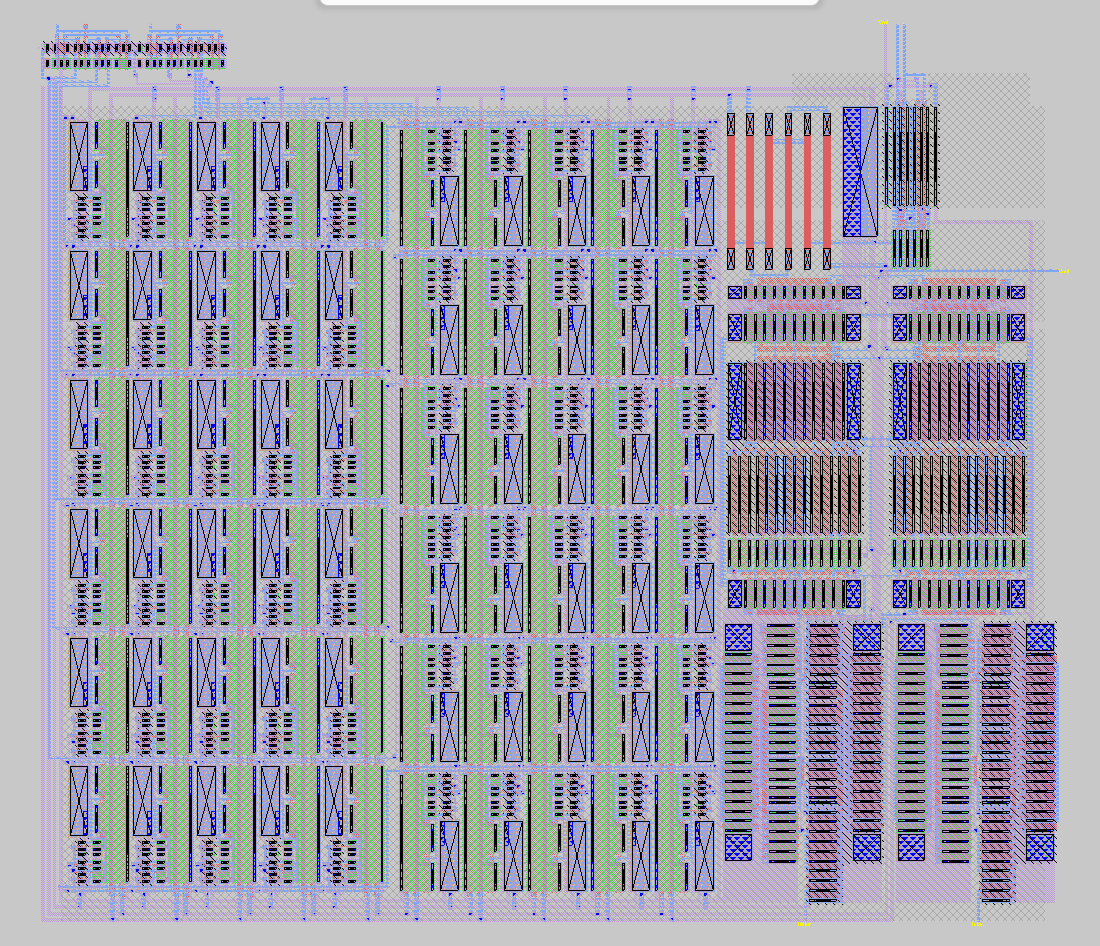
\includegraphics[width=0.7\columnwidth]{images/full_layout.png}
    \caption{full layout of the DAC, DAC controller, I-V converter, Output stage, Bias Generators (with the mimcap layer not shown)}
    \label{fig:opamp_schematic}
\end{figure}

\begin{figure}[H]
    \centering{}
    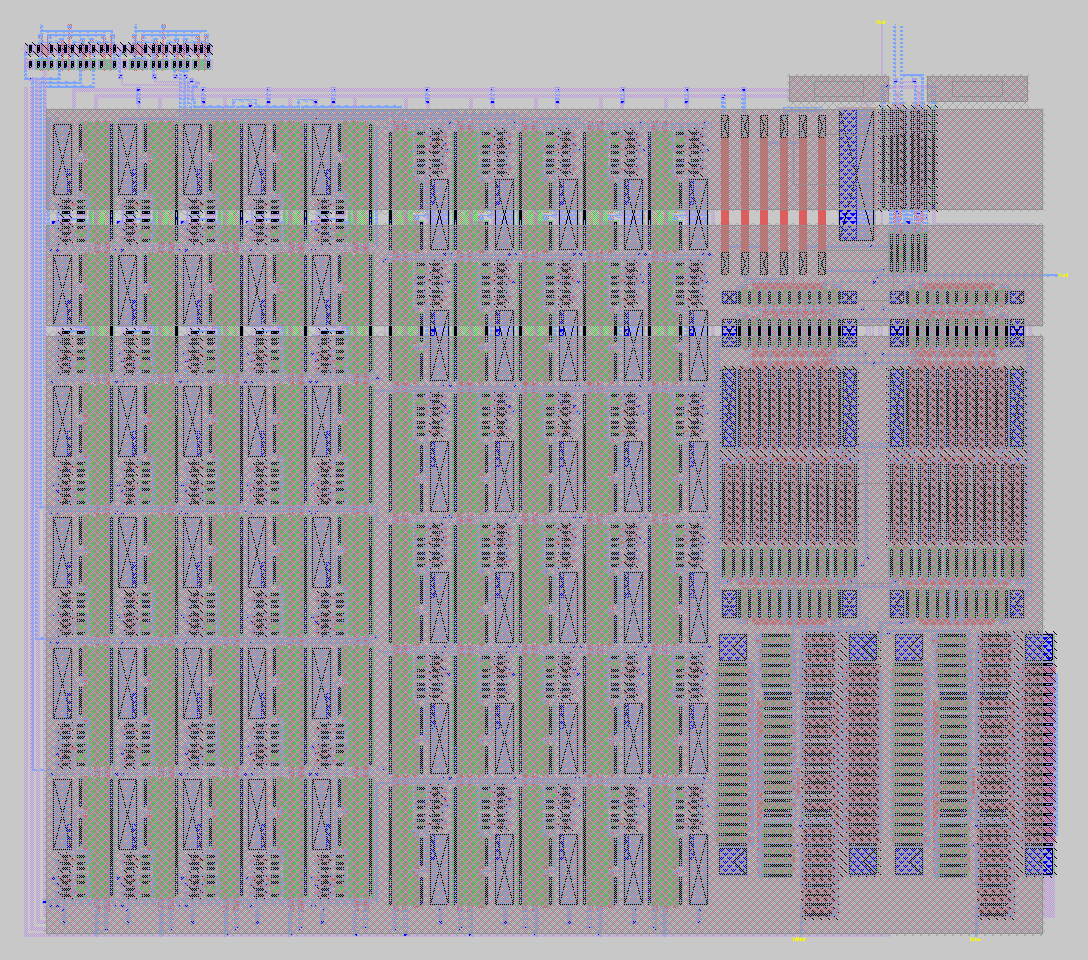
\includegraphics[width=0.7\columnwidth]{images/full_layout_showing_capacitors.png}
    \caption{full layout of the DAC, DAC controller, I-V converter, Output stage, Bias Generators (with the mimcap layer shown)}
    \label{fig:opamp_schematic}
\end{figure}


\end{document}